%\documentclass[11pt,a4paper,oneside]{report}             % Single-side
\documentclass[11pt,a4paper,twoside,openright]{report}  % Duplex

%\PassOptionsToPackage{chapternumber=Huordinal}{magyar.ldf}
\usepackage{t1enc}
\usepackage[latin2]{inputenc}
\usepackage{amsmath}
\usepackage{amssymb}
\usepackage{enumerate}
\usepackage[thmmarks]{ntheorem}
\usepackage{graphics}
\usepackage{epsfig}
\usepackage{listings}
\usepackage{color}
%\usepackage{fancyhdr}
\usepackage{lastpage}
\usepackage{anysize}
%\usepackage[magyar]{babel}
\usepackage[english,magyar]{babel}
\usepackage{sectsty}
\usepackage{setspace}  % Ettol a tablazatok, abrak, labjegyzetek maradnak 1-es sorkozzel!
\usepackage[hang]{caption}
\usepackage{hyperref}
\usepackage{subcaption}

%--------------------------------------------------------------------------------------
% Main variables
%--------------------------------------------------------------------------------------
\newcommand{\vikszerzo}{Velinszky L�szl�}
\newcommand{\vikkonzulens}{dr.~Strausz Gy�rgy}
\newcommand{\vikcim}{Monitoring Cyberphysical Systems}
\newcommand{\viktanszek}{Department of Measurement and Information Systems}
\newcommand{\vikdoktipus}{MSc Thesis}
\newcommand{\vikdepartmentr}{Velinszky L�szl�}

%--------------------------------------------------------------------------------------
% Page layout setup
%--------------------------------------------------------------------------------------
% we need to redefine the pagestyle plain
% another possibility is to use the body of this command without \fancypagestyle
% and use \pagestyle{fancy} but in that case the special pages
% (like the ToC, the References, and the Chapter pages)remain in plane style

\pagestyle{plain}
\setlength{\parindent}{0pt} % �ttekinthet�bb, angol nyelv� dokumentumokban jellemz�
\setlength{\parskip}{8pt plus 3pt minus 3pt} % �ttekinthet�bb, angol nyelv� dokumentumokban jellemz�
%\setlength{\parindent}{12pt} % magyar nyelv� dokumentumokban jellemz�
%\setlength{\parskip}{0pt}    % magyar nyelv� dokumentumokban jellemz�

\marginsize{35mm}{25mm}{15mm}{15mm} % anysize package
\setcounter{secnumdepth}{0}
\sectionfont{\large\upshape\bfseries}
\setcounter{secnumdepth}{2}
\singlespacing
\frenchspacing

%--------------------------------------------------------------------------------------
%	Setup hyperref package
%--------------------------------------------------------------------------------------
\hypersetup{
    bookmarks=true,            % show bookmarks bar?
    unicode=true,             % non-Latin characters in Acrobat�s bookmarks
    pdftitle={\vikcim},        % title
    pdfauthor={\vikszerzo},    % author
    pdfsubject={\vikdoktipus}, % subject of the document
    pdfcreator={\vikszerzo},   % creator of the document
    pdfproducer={Producer},    % producer of the document
    pdfkeywords={keywords},    % list of keywords
    pdfnewwindow=true,         % links in new window
    colorlinks=true,           % false: boxed links; true: colored links
    linkcolor=black,           % color of internal links
    citecolor=black,           % color of links to bibliography
    filecolor=black,           % color of file links
    urlcolor=black             % color of external links
}

%--------------------------------------------------------------------------------------
% Set up listings
%--------------------------------------------------------------------------------------
\lstset{
	basicstyle=\scriptsize\ttfamily, % print whole listing small
	keywordstyle=\color{black}\bfseries\underbar, % underlined bold black keywords
	identifierstyle=, 					% nothing happens
	commentstyle=\color{white}, % white comments
	stringstyle=\scriptsize\sffamily, 			% typewriter type for strings
	showstringspaces=false,     % no special string spaces
	aboveskip=3pt,
	belowskip=3pt,
	columns=fixed,
	backgroundcolor=\color{lightgray},
	breaklines=true,
	breakautoindent=true,
	breakatwhitespace=true,
} 		
\def\lstlistingname{Listing}	

%--------------------------------------------------------------------------------------
%	Some new commands and declarations
%--------------------------------------------------------------------------------------
\newcommand{\code}[1]{{\upshape\ttfamily\scriptsize\indent #1}}

% define references
\newcommand{\figref}[1]{\ref{fig:#1}.}
\renewcommand{\eqref}[1]{(\ref{eq:#1})}
\newcommand{\listref}[1]{\ref{listing:#1}.}
\newcommand{\sectref}[1]{\ref{sect:#1}}
\newcommand{\tabref}[1]{\ref{tab:#1}.}

\DeclareMathOperator*{\argmax}{arg\,max}
%\DeclareMathOperator*[1]{\floor}{arg\,max}
\DeclareMathOperator{\sign}{sgn}
\DeclareMathOperator{\rot}{rot}
\definecolor{lightgray}{rgb}{0.95,0.95,0.95}

\author{\vikszerzo}
\title{\viktitle}
\includeonly{
	guideline,%
	project,%
	titlepage,%
	declaration,%
	abstract,%
	introduction,%
	chapter1,%
	chapter2,%
	chapter3,%
	chapter4,%
	acknowledgement,%
	appendices,%
}
%--------------------------------------------------------------------------------------
%	Setup captions
%--------------------------------------------------------------------------------------
\captionsetup[figure]{
%labelsep=none,
%font={footnotesize,it},
%justification=justified,
width=.75\textwidth,
aboveskip=10pt}

\renewcommand{\captionlabelfont}{\small\bf}
\renewcommand{\captionfont}{\footnotesize\it}

%--------------------------------------------------------------------------------------
% Table of contents and the main text
%--------------------------------------------------------------------------------------
\begin{document}
\singlespacing

\pagenumbering{arabic}
\onehalfspacing
\selectlanguage{english}
%--------------------------------------------------------------------------------------
%	The title page
%--------------------------------------------------------------------------------------
\begin{titlepage}
\begin{center}

\includegraphics[width=60mm,keepaspectratio]{figures/BMElogo.png}\\
\vspace{0.3cm}
\textbf{Budapesti M�szaki �s Gazdas�gtudom�nyi Egyetem}\\
\textmd{Villamosm�rn�ki �s Informatikai Kar}\\
\textmd{\viktanszek}\\[5cm]

\vspace{0.4cm}
{\huge \bfseries \vikcim}\\[0.8cm]
\vspace{0.5cm}
\textsc{\Large \vikdoktipus}\\[4cm]

\begin{tabular}{cc}
 \makebox[7cm]{\emph{K�sz�tette}} & \makebox[7cm]{\emph{Konzulens}} \\
 \makebox[7cm]{\vikszerzo} & \makebox[7cm]{\vikkonzulens}
\end{tabular}

\vfill
{\large \today}
\end{center}
\end{titlepage}



\tableofcontents\vfill
%--------------------------------------------------------------------------------------
% Nyilatkozat
%--------------------------------------------------------------------------------------
\begin{center}
\large
\textbf{HALLGAT�I NYILATKOZAT}\\
\end{center}

Alul�rott \emph{\vikszerzo}, szigorl� hallgat� kijelentem, hogy ezt a  diplomatervet meg nem engedett seg�ts�g n�lk�l, saj�t magam k�sz�tettem, csak a megadott forr�sokat (szakirodalom, eszk�z�k stb.) haszn�ltam fel. Minden olyan r�szt, melyet sz� szerint, vagy azonos �rtelemben, de �tfogalmazva m�s forr�sb�l �tvettem, egy�rtelm�en, a forr�s megad�s�val megjel�ltem.

Hozz�j�rulok, hogy a jelen munk�m alapadatait (szerz�(k), c�m, angol �s magyar nyelv� tartalmi kivonat, k�sz�t�s �ve, konzulens(ek) neve) a BME VIK nyilv�nosan hozz�f�rhet� elektronikus form�ban, a munka teljes sz�veg�t pedig az egyetem bels� h�l�zat�n kereszt�l (vagy autentik�lt felhaszn�l�k sz�m�ra) k�zz�tegye. Kijelentem, hogy a beny�jtott munka �s annak elektronikus verzi�ja megegyezik. D�k�ni enged�llyel titkos�tott diplomatervek eset�n a dolgozat sz�vege csak 3 �v eltelte ut�n v�lik hozz�f�rhet�v�.

\begin{flushleft}
\vspace*{1cm}
Budapest, \today
\end{flushleft}

\begin{flushright}
 \vspace*{1cm}
 \makebox[7cm]{\rule{6cm}{.4pt}}\\
 \makebox[7cm]{\emph{\vikszerzo}}\\
 \makebox[7cm]{hallgat�}
\end{flushright}
\thispagestyle{empty}

\vfill
\clearpage
\thispagestyle{empty} % an empty page


%----------------------------------------------------------------------------
% Abstract in hungarian
%----------------------------------------------------------------------------
\selectlanguage{magyar}
\chapter*{Kivonat}\addcontentsline{toc}{chapter}{Kivonat}

Minden ember nap mint nap tal�lkozik olyan szenzorokkal, melyek h�l�zatba k�tve kommunik�lnak egym�ssal vagy egy k�zponti egys�ggel. Ezek lehetnek ak�r id�j�r�s �rz�kel�k, utcai kamer�k vagy mobiltelefonok. Az eszk�z�k  "Internet of things" (dolgok internetje) r�sz�v� v�lnak, hogy azt�n a m�r�seket ki�rt�kelve k�vetkeztet�seket vonjunk le, �s automatikusan beavatkozhassunk a k�rnyezet�nkbe. Az ilyen rendszereket h�vjuk kiberfizikai rendszernek. Ezek azonban t�bbnyire elszigetelt adatb�zisokb�l �llnak, ahol a k��nb�z\H{o} adatb�zisok k�z�tt nincs kapcsolat, s\H{o}t k�l�n�sebb el\H{o}nyt az �sszekapcsol�s sem jelentene. A szenzoradaok felett egy olyan le�r�s is sz�ks�ges ehhez, mely ezeket a szemantikai kapcsolatokat �rja le a szenzorok k�z�tt. A szemantikai kapcsolat megl�te eset�n k�vetkeztetni lehet sz�m�t�g�p seg�ts�g�vel az adatokb�l vagy k�nnyebb m�don lehet keresni az adatb�zisban. Az egyetemi projekt kapcs�n egy ilyen rendszer lett ki�p�tve, ehhez azonban t�bb dolog sz�ks�ges. 

Sz�ks�g van egy szab�nyos nyelvre, mely alapj�n a szenzoradatok lek�rdehet\H{o}ek a rendszerb\H{o}l, ez a nyelv az OGC konzorcium �ltal fenntartott SensorML. Ez egy XML alap� nyelv, melynek t�bb ny�lt forr�s� implement�ci�ja l�tezik. Ezek k�z�l az 52north az egyik legelterjedtebb �s legdinamikusabban fejl?d?, �gy ez lett felhaszn�lva az egyetemi projekt kapcs�n is.

A m�sik sz�ks�ges r�sz a szemantikai le�r�st megval�s�t� ontol�gia. Ennek t�rol�s�ra az RDF a leggyakrabban haszn�lt le�r�si  m�dszer. Az ontol�gia t�rol�s�ra is t�bb adatb�zis l�tezik, ezek k�z�l az egyetemi projekt a Stardog RDF adatb�zist haszn�lja, mely minden sz�ks�ge funkci�t integr�lva tartalmaz.

A FIRST r�vid�t�s? EU-s projekt keret�n k�sz�lt el, az ezen alkot�elemeket felhaszn�l� kiberfizikai rendszer. A rendszer k�pes az adatok szemantikai le�r�s�ra, a m�r�sek t�rol�s�ra �s �jabb alkalmaz�sok telep�t�s�re.

A m�rt adatokat felhaszn�l�s�hoz, a k�vetkeztet�sek levon�s�hoz sz�ks�ges egy monitoroz� rendszer, mely a felhaszn�l� sz�m�ra �rtelmezhet\H{o} form�ban jelen�ti meg a m�rt �rt�keket. Egy ilyen web alap�, mobilbar�t rendszer lett kialak�tva �s telep�tve a megl�v\H{o} rendszer mell�.  
%----------------------------------------------------------------------------
% Abstract in english
%----------------------------------------------------------------------------
\selectlanguage{english}
\chapter*{Abstract}\addcontentsline{toc}{chapter}{Abstract}

Most of us encounter different sensors every day that act together while connected into a network. These can be either weather sensors, CCTV cameras or smart-phones. These devices become part of the Internet of Things by evaluating their observations and interacting with its environment.
These are called cyberphysical systems. 
These systems usually contain separate databases, where each database is not connected with the others in any way, moreover the existence of these connections would not gain any advantage.
There should be such a description on top of the sensor data, which would describe such semantic connections between the sensors.
While having such a description it would be possible to reason with the help of a computer using the data or it would make searching the database easier. During the University project such a system was built, which required some additional things.

A standard language is needed, which makes querying, manipulating the data possible. This is SensorML, which is maintained by Open Geospatial Consortium. This is an XML based language which has many open source implementation. The most popular and rapidly developing one is 52north, which was used in the University project.

The other necessary part is the ontology which  is the semantic description of the system. The RDF standard is the most popular way to describe such properties. There are many RDF stores, from which the Stardog RDF has been used, which contains all necessary features integrated in an easy to use way.

The cyberpysical system was created within the EU project FIRST. The system is capable of storing the description and the measurements and it can deploy new applications too.

To use the measured data and see the conclusion a user friendly monitoring system shall be created. Such a WEB based, mobile friendly system was designed and deployed next to the cyberphysical system.

\vfill


%----------------------------------------------------------------------------
\chapter*{Introduction}\addcontentsline{toc}{chapter}{Introduction}
%----------------------------------------------------------------------------

Nowadays, most of our devices are connected through the Internet. Our computers, mobile phones, surveillance cameras share their information via the world wide web. Each device has many sensors, such as GPS, gravity, acceleration sensor, imaging devices or just processing powers. These sensors' or resources' information are stored individually on each device. 

The world is emerging into a state that information needs to be shared between peers and should be stored in an easy to reach independent location called Cloud. The Cloud is a distributed information store which can be reached through the Internet.
This enables sensor information to be stored and processed for new uses, because the same sensor can be used for different purposes. An outdoor surveillance camera can be used to protect from intruders or to provide weather information. This data can be used for different purposes in various regions. A local measurement can control the local heating system, but a grid of weather stations can be used to provide forecast data.
 
 It is not enough to measure all the data using such sensors. It has to be stored for analytics as it can be a source for predictions. Storing has become easier in the BigData world we live in. There are expectations of the method of storing the data. It should be transparent letting different systems share information with each other. To create such a standardized way of storing sensor measurement data Open Geospatial Consorptium started and maintains the SensorMl format. One of SensorML's couple layers is the SOS (Sensor Observation Service) which provides different ways to reach the observed data. This storage engine makes it available for outer services and inner services (like virtual sensors) to reach the desired data and run analytics and trigger monitoring events on them.

Storing sensor data does not give any semantic knowledge about the system. Such knowledge can be that a wind sensor is also a weather sensor or a camera is a visual sensor. To describe such semantic connections an ontology has to be created. There are many ways to store ontologies. Usually they are described as triples like in the most common RDF format but there are newer formats which have extended capabilities and can describe natively much more things (such as temporal logic) like OWL format. Storing such ontologies are done using special RDF databases. Such databases can analyze connections faster, it is even possible to gain new knowledge from predefined conditions using reasoning. This way we can describe such things that if an Anemometer is a kind of wind sensor, and wind sensors are weather sensors then without specifying explicitly that the Anemometer is a weather sensor the system already knows the answer. 

If we have such an enormous system it can be hard to maintain it. There can be thousands or even more sensors in a network with different capabilities and efficiency. The operation of the sensors should be monitored in an easy to access method where each sensor's state and measurements should be easy to reach via a modern user interface. The purpose of this document is to describe such a large system's architecture and to provide a tool with which a monitoring task can be done.

Such a system is described in this paper. The chosen format is a dynamic, interactive web page. The page consists of an engine that is capable of showing the measurements and state of the sensors using both the RDF and the SOS databases. The sensors' measurements are displayed on a user friendly page. The sensors can be filtered to show only a group of sensors. A status page for the failures are also included to have a big picture of the state of the system. These pages can be viewed from any device such as PCs, tablets or mobile phones.

In the next two section the basics of the used technologies are described. First, there is a detailed introduction to the SOS server and the SensorML standard. After that the semantic description language and its storage engine are introduced. 
In the third chapter, the actual system is shown what the monitoring supports. 
There will be a detailed introduction to the components and the used sensors, and some use cases for the system. The final chapter describes the monitoring system in details. It shows its structure, the used third party frameworks and a usage manual. In the end, the whole work will be summarized. 


%----------------------------------------------------------------------------
\chapter{Introduction of SensorML and SensorWeb}\label{sect:Introduction}
%----------------------------------------------------------------------------
\section{Goals of observation gathering}
%----------------------------------------------------------------------------
Most phyisical quantities are measured with great accuracy on very basic devices. From the most basic sound measurements with microphone, to the nowadays popular inertial measurement units every data can be measured. There are also weather sensors and solar sensors available for everyone.

 With the evolution of sensor fusion algorithms these data can be merged together to give an even better accuracy or a general knowledge of our environment. This data can be used to predict weather conditions by merging neighborhood sensors into one. It can be used to make predictions based on the weather conditions in an area and the direction of the wind on the location.
 
 \begin{figure}[h]
 \centering
 %http://www.crystaldatainternational.com/choices/sensorml.html
  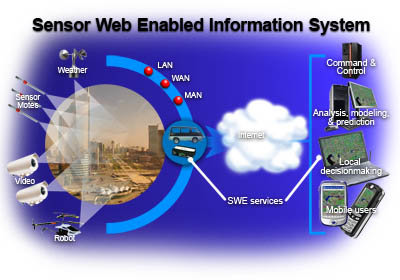
\includegraphics[width=0.6\textwidth]{figures/webswe.png}
 \caption{SWE architecture\label{fig:webswe}}
 \end{figure}
 
 
 The other challenge is to use a sensor's data for multiple purposes. For example a CCTV camera picture can be used to count the number of cars on the road, to get an estimation of the speedings in a crossing or to get visual weather data. Computer Vision algorithms, regressions and special machine learning algorithms need different computing resources. Those can be outsourced to different computers which must have access to the data. The Sensor Observation Server is used to make this all available.
 
 \section{Types of sensors}
 
 Sensors are all around us. We have sensors in our cell phones or any handheld devices. Most of them are connected to the internet or a network. The measurements of all of these devices can be stored and queried from a database. The usable data in some devices are:
 
 \begin{itemize}
 	\item Smartphone
 	 \begin{itemize}
	 	 \item Camera: Visual image of the phone itself
	 	 \item Accelerometer: measurement of the acceleration of a system. Derivate of speed.
	 	 \item Weather sensors: Often smartphones has built in temperature sensors, rarely barometer is also installed.
	 	 \item Computing resource: ability to run additional softwares by using up its resources
	 	 \item Gyroscope: Orientation sensor.
 	 \end{itemize}
 	 \item Weather sensor
 	 \begin{itemize}
 	 \item Tempareture sensor: Inner and outer temperature.
 	 \item Humidity sensor: percentage of humidity.
 	 \item Barometer: Air pressure.
 	 \end{itemize}
 	 \item Beagleboard
 	 \begin{itemize}
	\item Computing resource.
 	 \end{itemize}
 \end{itemize}

The examples show that a standard way to retrieve the measurements should include not only the measurement, but the type of the sensor, the measured unit, the location of the sensor and many additional information like this. 

Storing and retrieving this information is done using the SensorML format.

\section{The SensorML}

The Open Geospatial Consortium approved the SensorML language to be able to describe all the necessary information about measured data\cite{sensorml}. This is an XML based language that is used to describe the sensors, add, update, delete or retrieve information. The SensorML is able to solve the above mentioned problems. It is an abstract definition of the sensor information.

To have a general structure for the data, there is an abstract hierarchy that represents sensors and measurements. They have their own concepts which is described in as follows \cite{g2d2}:
\begin{itemize}
\item FeatureOfInterest: additional constraints provided for the measurement, e.g. time or location of measurement.
\item ObservedProperty: what type of physical property is measured, e.g. speed, temperature.
\item Procedure: the virtual or real sensor itself that is providing the data.
\item Offering: the property itself that has been measured, e.g. wind speed, air humidity, traffic size. 
\item Result: the output of the procedure.
\end{itemize}

This way gives as enough abstraction to separate the measured properties, the physical properties, the actual sensors and the results from each other.

It is able to define the location of the sensor, the timestamp of the measurement and the sensor data itself, with many additional information. The data can be stored in SOS servers that can retrieve the data on different interfaces.
 
\section{Server Observation Service}

Server Observation Servers store SensorML data and let others query, manipulate and add sensors to the database. These sensors can be derived sensors. Such derived sensors are called procedures. A procedure can be a traffic information based on the CCTV camera. An SOS server should be able to handle dependencies based on which procedure requires other procedures to provide data. Sometimes derived sensors are also called virtual sensors, because they don't do physical measurement but provide a derived value.

There are many closed and open source implementations of SOS servers. Some open source implementations are introduced here.

The MapServer is written in C, C++, however it can be extended in many other languages\cite{mapserver}. It has a built in GUI to view data, however it is not yet available for the SOS implementation. The server can only be reached by one interface. It was originally developed by University of Minnesota. In the time of writing the paper the code is maintained and supported by the Open Source Geospatial Foundation. It is mostly used for mapping not for serving data for derived sensors. It was used in some projects between NASA and the University of Minnesota. 

istSOS is another implementation in Python\cite{istsos}. It runs its scripts from Apache web server just like MapServer. It uses PostgreSQL database backend to store values. It has a nice GUI for administration. Only supports standard SensorML interface to retrieve data. It is a project of the SUPSI University in Switzerland.

OOSThetys is a basic toolkit for enabling SensorML communication. It is written in Perl and Java. It is fairly documentated and seems to be abandoned because there has been no new release since the February of 2012.

52north SOS is a sample implementation written in Java\cite{52north}. It runs as a web service from Apache tomcat to serve requests. It also uses PostgreSQL with PostGIS extension. The application is used in the sample implementation and it is covered in details later.

All SOS servers and the whole SensorML standard is missing the semantic information about the sensors meaning that all sensor data are stored in such a database and all properties can be described for the sensors but no connection between the concepts can be described for the sensor.

\section{52north SOS server}

This implementation is done by the non profit organization with the identical name. The software supports many interfaces to query the information needed. The standard SOAP can be used to work with Java Web services. There are KVP and POX to retrieve or add data using standard GET queries. A big advantage is that 52north SOS supports JSON interface. It enables JSON queries to retrieve information efficiently in JavaScript, PHP, Python or other modern scripting languages.

The new 4.2 version is easy to install, it has a graphical user interface to set up the database connection and initialize the database. PostgreSQL with PostGIS is required.  The basic usage is described on  52north webpage, but sample queries are shown in the built in test client. 

The project is built with Maven and uses Spring framework too. The included unit tests ensure that the software's architecture is still consistent after compilation. The project was chosen to be part of Google's Summer of Code 2014 and the project gained a lot improvements from that. 

A request can be sent using the connector of each interface. This used to be done by adding the interface name to the application url but in recent versions the service automatically detects the interface from the HTTP metadata. For example http://152.66.253.152:8080/52n-sos-webapp/service is the url where all interface can be reached. The first part is the host of the server. The tomcat application server is listening on port 8080. 52n-sos-webapp is the default name of the web application, service it the default connector for the webservice. The sent HTTP content-type header marks the interface. A detailed description of the interfaces can be seen on table \ref{tab:services}.
\begin{table}[h]
\begin{center}
\begin{tabular}{| l | l | p{8cm} |}
\hline
Interface  & Content type & Description \\ \hline \hline
SOAP & application/soap+xml & Standard SOAP request mostly used in JAVA, it is sending the request in XML format using POST request. \\ \hline
POX & application/xml & Very similar to SOAP but has a different XML format. \\ \hline
KVP & application/xml & This is a GET request, meaning that all request parameters are encoded in the URL. The answer is in XML format. \\ \hline
JSON & applicaton/json & This is a POST request which sends and receives information using JSON objects. Most programming languages can easily parse this type of request.\\ \hline
\end{tabular}
\caption{Interfaces for 52n SOS server\label{tab:services}}
\end{center}
\end{table}


\section{SOS commands}
There are many commands to query or manipulate the SOS server. In this section some of them will be shown using the JSON interface. 

The GetCapabilities command (shown on listing \ref{lst:getcap}) allows the clients to retrieve a list of the reachable sensors of the server and their configuration. This command lists all the available measurements on the server too. This call does not have any required parameters, only if the details of the response should be controlled. Such detail is the section to be displayed. There are 4 different sections:
\begin{itemize}
\item ServiceIdentification: the list of profiles that the server has been using. These profiles describe the format that the data is represented in.
\item ServiceProvider: in this section is the contact information for the operator of the SOS service.
\item OperationMetadata: this section provides the available options and their possible values.
\item FilterCapabilities: what fields are available for filtering. Can be spatial filtering for location or temporal filtering for time range.
\item Contents: summary of the type and FOI of each procedure. 
\end{itemize}

\begin{lstlisting}[caption={JSON getCapabilities POST request\label{lst:getcap}}]
{
  "request": "GetCapabilities",
  "service": "SOS",
  "sections": [
    "ServiceIdentification",
    "ServiceProvider",
    "OperationsMetadata",
    "FilterCapabilities",
    "Contents"
  ]
}
\end{lstlisting}

 If the procedure is known the DescribeSensor command will describe the measurements of the selected sensor. The response will include a description field which contains the details about the sensor in the standard XML based SensorML format. The sample request code can be seen on listing \ref{lst:descsens}.

\begin{lstlisting}[caption={JSON DescribeSensor POST request\label{lst:descsens}}]
{
  "request": "DescribeSensor",
  "service": "SOS",
  "version": "2.0.0",
  "procedure": "http://www.52north.org/test/procedure/1",
  "procedureDescriptionFormat": "http://www.opengis.net/sensorML/1.0.1"
}
\end{lstlisting}

After knowing the necessary parameters the getObservation property can be called. This command shows the measured values for some given observations. The input can be complex, it can filter based on procedures, offerings, observed properties, on any feature of interest or temporal or spatial filters. A sample can be read from listing \ref{lst:getobs}.

\begin{lstlisting}[caption={JSON GetObservation POST request with all filters\label{lst:getobs}}]
{
  "request": "GetObservation",
  "service": "SOS",
  "version": "2.0.0",
  "procedure": [
    "http://www.52north.org/test/procedure/6",
    "http://www.52north.org/test/procedure/1"
  ],
  "offering": [
    "http://www.52north.org/test/offering/6",
    "http://www.52north.org/test/offering/1"
  ],
  "observedProperty": [
    "http://www.52north.org/test/observableProperty/1",
    "http://www.52north.org/test/observableProperty/6"
  ],
  "featureOfInterest": [
    "http://www.52north.org/test/featureOfInterest/6",
    "http://www.52north.org/test/featureOfInterest/1"
  ],
  "spatialFilter": {
    "bbox": {
      "ref": "om:featureOfInterest/sams:SF_SpatialSamplingFeature/sams:shape",
      "value": {
        "type": "Polygon",
        "coordinates": [
          [ [ 50, 7 ],
            [ 53, 7 ],
            [ 53, 10],
            [ 50, 10],
            [ 50, 7 ]
          ]
        ]
      }
    }
  },
  "temporalFilter": [
    {
      "during": {
        "ref": "om:phenomenonTime",
        "value": [
          "2012-11-19T14:00:00+01:00",
          "2012-11-19T14:05:00+01:00"
        ]
      }
    },
    { 
      "equals": {
        "ref": "om:phenomenonTime",
        "value": "2012-11-19T14:08:00+01:00"
      }
    }
  ]
}
\end{lstlisting}

The response (on listing \ref{lst:sendobs}) will contain the usual header which is contained by all the responses. It tells the requester the version of the response. After that comes the list of the observations that fit the conditions given. In the observation objects there are the procedures that measured the result, the feature of interests and the observable property that has been measured. The result object contains the uom field which is an abbreviation for the unit of measurement and the specific value. It can be an integer value, floating point or some encoded binary data.

\begin{lstlisting}[caption={JSON GetObservation response\label{lst:sendobs}}]
{
    "request": "GetObservation",
    "version": "2.0.0",
    "service": "SOS",
    "observations": [
        {
            "type": "http://www.opengis.net/def/observationType/OGC-OM/2.0/OM_Measurement",
            "procedure": "http://www.52north.org/test/procedure/6",
            "offering": "http://www.52north.org/test/offering/6",
            "observableProperty": "http://www.52north.org/test/observableProperty/6",
            "featureOfInterest": {
                "identifier": {
                    "codespace": "http://www.opengis.net/def/nil/OGC/0/unknown",
                    "value": "http://www.52north.org/test/featureOfInterest/6"
                },
                "sampledFeature": "http://www.52north.org/test/featureOfInterest/world",
                "geometry": {
                    "type": "Point",
                    "coordinates": [
                        51.447722,
                        7.270806
                    ]
                }
            },
            "phenomenonTime": "2012-11-19T13:09:00.000Z",
            "resultTime": "2012-11-19T13:09:00.000Z",
            "result": {
                "uom": "test_unit_6",
                "value": 2.9
            }
        },
        {
            "type": "http://www.opengis.net/def/observationType/OGC-OM/2.0/OM_Measurement",
            "procedure": "http://www.52north.org/test/procedure/6",
            "offering": "http://www.52north.org/test/offering/6",
            "observableProperty": "http://www.52north.org/test/observableProperty/6",
            "featureOfInterest": {
                "identifier": {
                    "codespace": "http://www.opengis.net/def/nil/OGC/0/unknown",
                    "value": "http://www.52north.org/test/featureOfInterest/6"
                },
                "sampledFeature": "http://www.52north.org/test/featureOfInterest/world",
                "geometry": {
                    "type": "Point",
                    "coordinates": [
                        51.447722,
                        7.270806
                    ]
                }
            },
            "phenomenonTime": "2012-11-19T13:03:00.000Z",
            "resultTime": "2012-11-19T13:03:00.000Z",
            "result": {
                "uom": "test_unit_6",
                "value": 2.3
            }
        }
    ]
}
\end{lstlisting}

If only the result fields are important to the user the shorter GetResult command can be used. It is shown on figure \ref{lst:getresult}.

\begin{lstlisting}[caption={JSON minimal GetResult POST request\label{lst:getresult}}]

{
  "request": "GetResult",
  "service": "SOS",
  "version": "2.0.0",
  "offering": "http://www.52north.org/test/offering/6",
  "observedProperty": "http://www.52north.org/test/observableProperty/6"
}
\end{lstlisting}

The response will be a list of values of the last measurement for the queried properties. The results will be given as a concatenated string where each measurement is separated by a comma and in each measurement the value and its timestamp is separated by a hash mark. It can be seen on figure \ref{lst:sendresult}.

\begin{lstlisting}[caption={JSON GetResult response\label{lst:sendresult}}]
{
    "request": "GetResult",
    "version": "2.0.0",
    "service": "SOS",
    "resultValues": "10#2012-11-19T13:00:00.000Z,2012-11-19T13:00:00.000Z,2.0#2012-11-19T13:01:00.000Z,2012-11-19T13:01:00.000Z,2.1#2012-11-19T13:02:00.000Z,2012-11-19T13:02:00.000Z,2.2#2012-11-19T13:03:00.000Z,2012-11-19T13:03:00.000Z,2.3#2012-11-19T13:04:00.000Z,2012-11-19T13:04:00.000Z,2.4#2012-11-19T13:05:00.000Z,2012-11-19T13:05:00.000Z,2.5#2012-11-19T13:06:00.000Z,2012-11-19T13:06:00.000Z,2.6#2012-11-19T13:07:00.000Z,2012-11-19T13:07:00.000Z,2.7#2012-11-19T13:08:00.000Z,2012-11-19T13:08:00.000Z,2.8#2012-11-19T13:09:00.000Z,2012-11-19T13:09:00.000Z,2.9"
}
\end{lstlisting}

There are other commands that manipulate the database, like InsertSensor, DeleteSensor to add or remove sensors. There are commands to add observable properties, and add results to the database too. 

\section{SOS client applications}

52north has a client application for the SOS server called 52n Sensorweb Client. This is a Java web application that can be configured to connect to multiple hosts and display their sensor data on maps and charts. It is developed using the same tools as the SOS server. This client is a web application which is can be opened in a web browser, but some parts run on the web server. This is a relatively complex application that does not yet understand semantic connections between the procedures. A screenshot can be seen on figure \ref{fig:sweclient}.

\begin{figure}[h]
\centering
%http://sensorweb.forum.52north.org/SWE-Client-Could-not-get-procedure-details-url-caused-by-java-lang-NullPointerException-td4025524.html
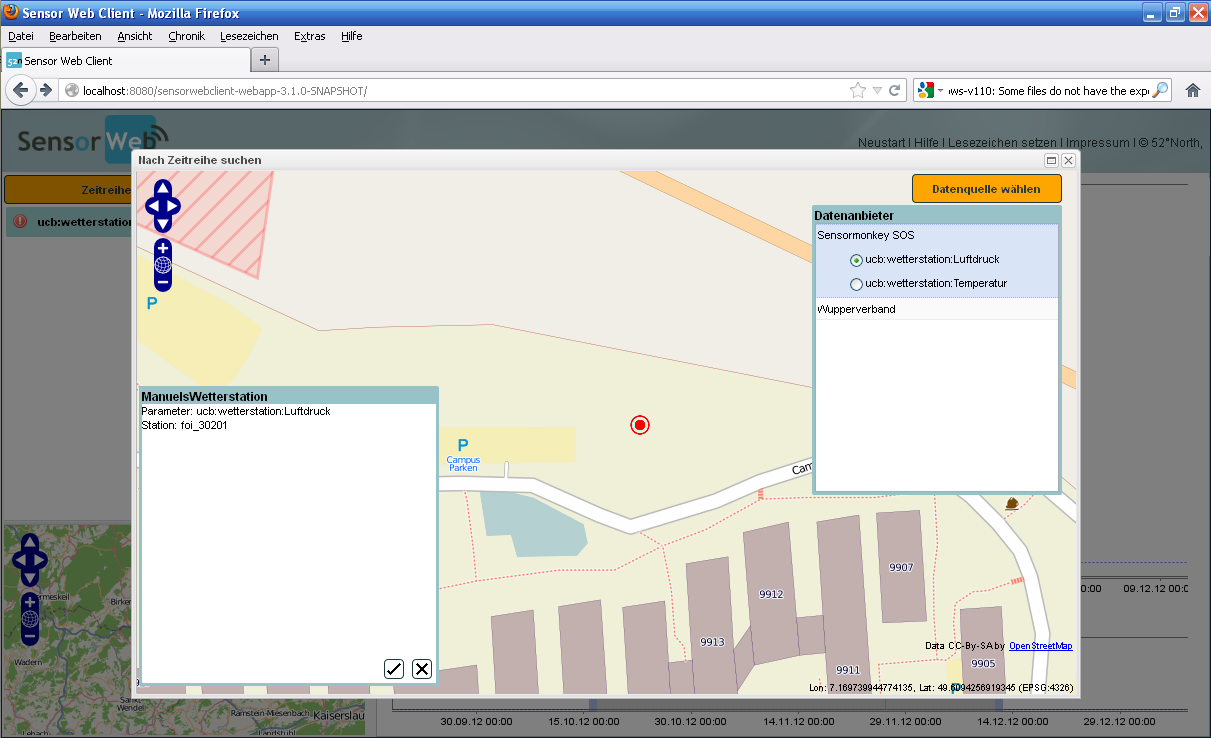
\includegraphics[width=0.6\textwidth]{figures/sweclient.png}
\caption{Screenshot of SWE Client 3\label{fig:sweclient}}
\end{figure}

There is a JavaScript framework that enables users to use only client side tools to connect to SOS servers and display data called SOS.js. Unfortunately, because of security restrictions on JavaScript cross-site request the data cannot be retrieved from the SOS server directly, the client has to be served from the same domain as the server. This is often not doable. That is why this application needs a proxy that forwards the data to the same domain to bypass this restriction. Screenshot can be seen on figure \ref{fig:sos-js}.

\begin{figure}[h]
\centering
%http://blog.52north.org/2014/02/21/sos-js/
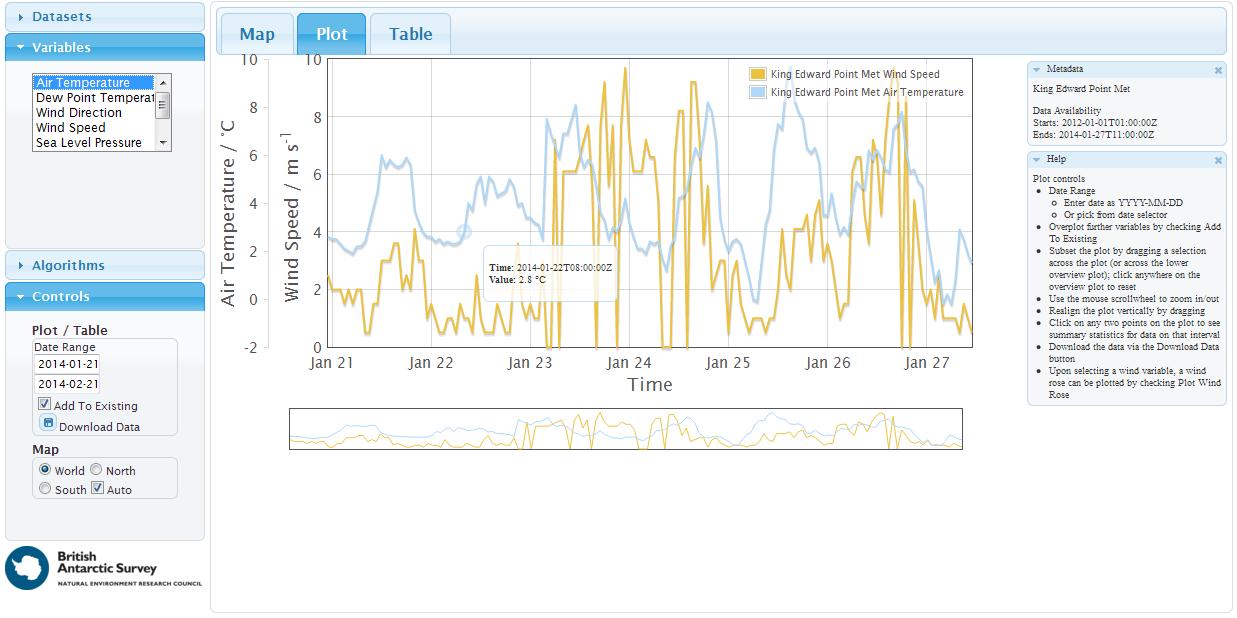
\includegraphics[width=0.6\textwidth]{figures/sos-js.png}
\caption{Screenshot of sos.js\label{fig:sos-js}}
\end{figure}

There are external softwares that can display their own measurements but not the SensorML standard. To make them usable with 52north SOS the developers created tools to extend such existing softwares to be able to import data from SOS. Such extension is the ArcGIS extension which makes SOS data available to ArcGIS server. This is also available to other programs such as $\mu$Dig. 

There are other tools to export data to R language or to use with other Geographic Information Systems (GIS) softwares. However, the problem is that no client software has the ability to make search available by semantic connections. A client has to be extended with such information to enable convenient filtering when monitoring a cyberphisical system.



\chapter{Semantic Connection}

\section{Advantages of semantic information}

\begin{figure}[h]
\centering
%self
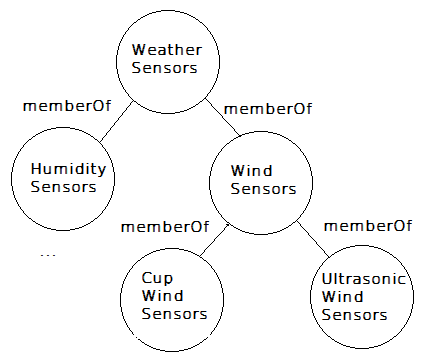
\includegraphics[width=0.6\textwidth]{figures/semws.png}
\caption{Using triples in the example\label{fig:semws}}
\end{figure}

In a cyberphisical system stored in an SOS every sensor has a name and a type. These are identifiers that correspond to a sensor and there may be other descriptors that are not informative for human reader. Sensors can be called on different names like Anemometer, Wind instrument, wind meter that means the same, measures the speed of the wind. Filtering for name is not a good approach for filtering the information. To make monitoring simpler. A semantic information is needed that organizes the data in a way that is convenient for the human reader to read. The sensors should be separated into different groups and subgroups and these groups should have an easily distinguishable name. Such groups can be Phyisical sensors -> Weather Sensors -> Wind sensors -> Wind speed sensors. This information yet can not be stored on the SOS server a separate ontology database shall be created. 
The usual way to store such information is in an ontology. 
An ontology is a description where objects, their properties and the connections between objects are described. This is very similar to classes, instances and relations in object oriented programming. An example of Java classes translated to an RDF ontology can be seen on Figure \ref{fig:rdf}\cite{g2d4}.


\begin{figure}
        \centering
        \begin{minipage}[b]{0.4\textwidth}
\begin{verbatim}

// classes
class Style {
 String neve;
}
class MusicalStyle 
	extends Style {
}
class Author {
 MusicalType musicalType;
}
// instances
MusicalType classic
 = new MusicalType();
Author Mozart =
 new Author();
Mozart.style = classic;
\end{verbatim}

        \end{minipage}
        \begin{minipage}[b]{0.4\textwidth}
        \begin{verbatim}

<!-- classes -->
<rdfs:Class rdf:id="Style"/>
<rdfs:Class rdf:id="MusicalStyle">
 <rdfs:subClassOf rdf:resource="#Style"/>
</rdfs:Class>
<rdfs:Class rdf:id="Author"/>
<!-- attributes -->
<rdf:Property rdf:id="StyleName">
 <rdfs:domain rdf:resource="#Style"/>
 <rdfs:range STRING/>
</rdf:Property>
<rdf:Property rdf:id="musicalStyle">
 <rdfs:domain rdf:resource="#Author"/>
 <rdfs:range rdf:resource="#MusicalStyle"/>
</rdf:Property>
<!-- instances -->
<MusicalStyle rdf:id="classic"/>
<Author rdf:id="Mozart">
 <MusicalStyle rdf:resource="#classic"/>
</Author>               
\end{verbatim}

        \end{minipage} 
 \caption{Java classes and their RDF representation side by side}
                \label{fig:rdf}
\end{figure}
The most widespread ontology storage standards are the RDF databases.

\section{Resource Definition Framework}

The RDF standard\cite{rdf} is created to be used with the Semantic Web approach to expand web pages with additional meanings that makes machines capable of understanding and reasoning about a web page. For example a web store can be easily understood by a customer: it has items, prices, shipping information, etc. However, for machines without saying explicitly that the value in one field is the price in USD it can be easily confused by the dimensions or the performance. Although nowadays these problems can be solved by machine learning, it is still a resource intensive process. To solve this problem an XML based standard has been introduced. In each page the data is explained using metadata information which is stored righ next to the HTML page itself. The pages can be directly referenced using their URL-s and anchors. The description is very simple, this is done by using triples. 

The triple describes \textit{which} page or entity (subject) is connected on \textit{what} property(predicate) to \textit{which} other page or entity(object). These subject, predicate and object triples are separate three unique values and it is called a statement.
Each value could have another triple describing it. The first (subject) part is the resource  which we make statements from. The second parameter (predicate) is the property of the resource that represents the attribute, aspect or connection. The third parameter is the value(object) which can refer to other resources or it can be a value from a specific domain like a number. This is very similar to statements in real life, like:
\begin{itemize}
\item Anemometer measures wind-speed
\item Anemometer is a wind-sensor
\item Wind-sensor is a sensor
\end{itemize} 
From the above example direct connections between wind-sensors and Anemometer can be described. Using reasoning indirect connections can be deduced. This makes RDF databases a powerful schema to describe real world examples. To be able to describe a big ontology which were put together using multiple ontologies each unique resource identifier is a fully qualified domain name and a hash tag and a unique name, like a URL with an anchor on a web page. 
The original idea behind the fully qualified domain name is that the approach was designed to give semantic meanings for web pages. 
Pages could refer to each other and give a global knowledge that is understandable by computers too. 

Such recursive data can be represented in graph databases, where reasoning is only walking in the database. There are graph databases to store these triples and also dedicated RDF databases. The standard way to query RDF databases is using SPARQL queries. Although RDF can represent data and connections it can not describe the rules how the reasoning, the walks in the graph should be done. These are represented by OWL or SWRL which are an extension to the RDF. However, most RDF databases also support such rules.

Raw RDF descriptor files are stored in XML format. A comparison beween classes and their RDF representation can be seen on \ref{fig:rdf}.


\begin{figure}[h]
\centering
%http://blog.52north.org/2014/02/21/sos-js/
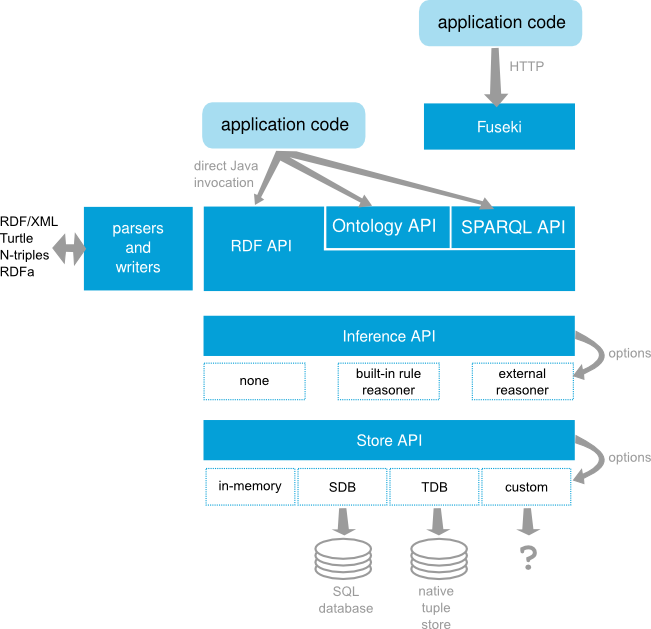
\includegraphics[width=0.6\textwidth]{figures/jena-architecture.png}
\caption{Architecture of Apache Jena\label{fig:jena}}
\end{figure}


\section{Some open source RDF databases} 

Apache Jena is an open source RDF datastore supported by the Apache foundation. It is written in Java\cite{jena}. It has many interfaces and supports many database backends. It can be used with in memory databases, SQL RDBs, triplestores. There is a built-in reasoner in the datastore, however it can be changed to other external reasoners too. The architecture of the software is shown on Figure \ref{fig:jena}.

OpenRDF Sesame is another tool for storing RDF triples. It is also written in Java. It has three different interfaces for communication: the SAIL API, the RIO interface and an HTTP client. The whole application runs from a Java container like Tomcat.

Apache Foundation also supports another RDF and Graph related project called Apache Marmotta. It was started in 2012. It supports a wide range of datastore engines from in memory databases through SQL servers to large distributed column bases stores like Apache Cassandra. 

There is an out of the box tool that contains better reasoners, has a basic GUI and accepts different data types. This is Stardog database. It is a commercial application. However, it has a community version with a few restrictions. The software is written in Java and run from a web container, like Tomcat. It supports many interfaces such as HTTP and SNARL, it has a built in reasoner with integrated constraint validation. Connectors for different programming languages are ready to use. It can be easily queried using SPARQL. It has support for OWL 2 rules. Because it is an easy to use, out of the box tool this database  is used in the sample application.

\begin{figure}[h]
\centering
%http://openrdf.callimachus.net/sesame/2.7/docs/articles/figures/sesame-components.png
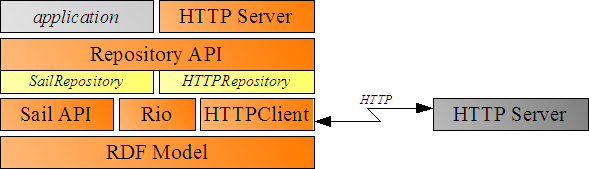
\includegraphics[width=0.6\textwidth]{figures/sesame-components.png}
\caption{Components of Sesame\label{fig:sesame}}
\end{figure}

\section{SPARQL for the queries}

To retrieve the necessary metadata the SPARQL query language is used in the RDF databases. These queries are less human readable than standard SQL queries, although they look similar. The language builds on the subject-predicate-object triples. In a result all matching data is responded. 

\begin{lstlisting}[caption={Sample SPARQL that queries all filterable objects\label{lst:sparql}}]
select ?s { <uri#filterable> <uri#subPropertyOf> ?s }
\end{lstlisting}

A SPARQL query can be quite complex. A simple query can be seen on listing \ref{lst:sparql}. A query can start with a BASE attribute, which defines the default prefix for each attribute. When this base is defined, it can be neglected from the query itself. As these are usually long URL-s, this can have a big gain on query length. The second given attributes are the prefixes. If external nodes from external sources are referenced, it can be shortened by using a prefix. This also results a shorter query. The next given parameter can be after a SELECT keyword a list separated by commas of the fields that should be displayed in the output. These are the variables that have been used in the condition. 
The condition part starts with the WHERE keyword. After that comes a multiple list of triples, where one keyword is either displayed in the result or have a reference in the query chain. Two triple can be either connected with a comma, a semi-colon or a dot. If it is a dot it means that the statement is finished the subject, predicate, object values are given. Having a semi-colon as a separator means that the subject should be repeated, only the predicate and the object is needed. The comma repeats the subject and the predicate, this way only the other object is needed. The prefix is separated by a colon from these values. Filtering functions can be also given in a query. For example the FILTER function can have one parameter and a regular expression and it filters only those values which fulfill the given regular expression. It can also compare values. Results can be grouped, ordered, just like in standard SQL languages. Aggregation of results are also possible. 

Predicates can be also used for recursive search. Listing every node of a subtree or leafs can be easier done in SPARQL. For selecting all the nodes, including the original, an asterisk has to be added to the end of the predicate. A plus sign will list every child element of the subject. These are called property paths and they are in the standard since version 1.1.

A SPARQL query can also provide other answers than returning a list of the answers. SELECT can be replaced by CONSTRUCT for creating new triples or by ASK which will check if the value exists in the repository. 


\begin{lstlisting}[caption={Sample complex SPARQL which shows top 5 countries based on population using DBpedia\label{lst:sparqlcomplex}}]
PREFIX type: <http://dbpedia.org/class/yago/>
PREFIX prop: <http://dbpedia.org/property/>
SELECT ?country_name ?population
WHERE {
?country a type:LandlockedCountries ;
rdfs:label ?country_name ;
prop:populationEstimate ?population .
FILTER (?population > 15000000 && langMatches(lang(?country_name), "en")) .
} ORDER BY DESC(?population) LIMIT 5
\end{lstlisting}

With such technology the triples can be stored and retrieved. However, the ontology behind the measurement is still missing. For that there is a standard ontology for sensors maintained by the Semantic Sensor Network Incubator Group. The underlying system which will be introduced in the next chapter is using this ontology in a somewhat customized way\cite{g2d2}.  The ontology is described in the next section.

\section{The Semantic Sensor Network Ontology}

The Semantic Sensor Network Incubator Group is a W3C incubator project. These projects are ran for one year to work on an area, this project ran from March of 2009 to September of 2010. It has developed an ontology for the semantic annotation of the Sensor Web Enablement standard. The ontology is available at http://www.w3.org/2005/Incubator/ssn/ssnx/ssn website, and it is conceptually organized into 10 modules. This is only a conceptual representation, the implementation consists of 41 concepts and 39 object properties. It is built upon a lightweight ontology, the  DOLCE-UltraLite. This underlying ontology helps the new one to connect with other semantic databases and to have a better understanding of the concepts behind the properties. 


\begin{figure}[h]
	\centering
	%custom
	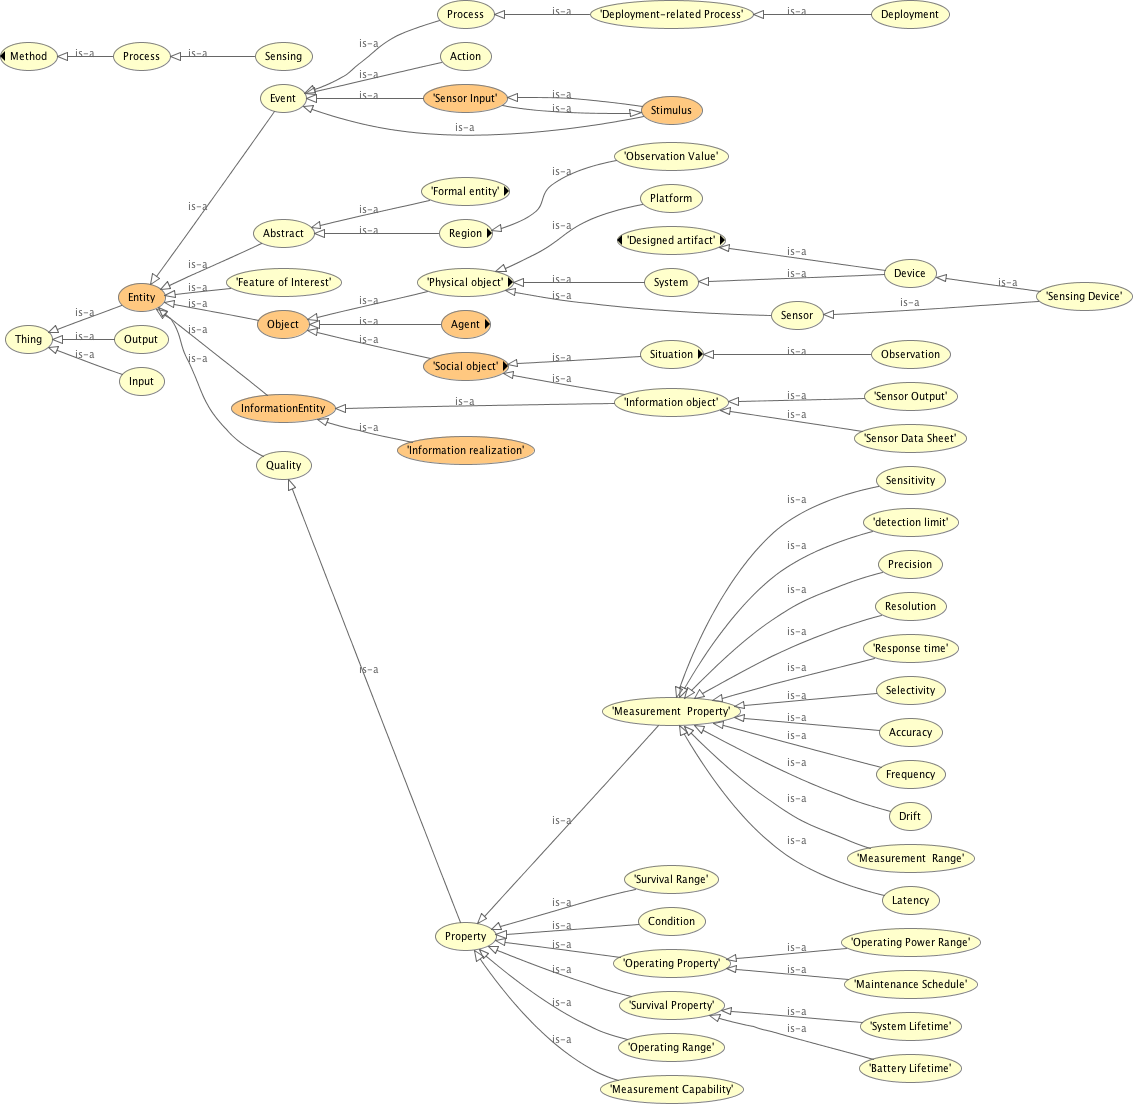
\includegraphics[width=0.9\textwidth]{figures/ssno-infer.png}
	\caption{Inferenced connections of the SSNO\label{fig:ssninfer}}
\end{figure}

The ontology can be viewed from four different perspectives:
\begin{itemize}
\item A sensor perspective with focus on what and how it senses and what it sensed.
\item An observation perspective which focuses on the observation and its environment.
\item A system perspective in focus on the network itself and the deployment.
\item A feature and property perspective which focuses on the physical properties and the subject of the observation. 
\end{itemize}
This makes it possible not just to deduct that for example wind sensor is a kind of sensor but that wind speed is a speed measurement. The connections between each object of the SSN ontology using reasoning can be seen on Figure \ref{fig:ssninfer}. 
In every ontology the ancestor is the Thing object. Its descendants are the Entities and the Input and Output objects. An entity can be an Event, like a measurement (sensor input), a process or an action. A sensor input is triggered by a Stimulus (stimulation of the sensor). The properties of the sensors are also Entities. There are two kind of properties, one is the property of the measurement and the other is the property of the sensor itself.


%----------------------------------------------------------------------------
\chapter{The used cyberphysical system}
%----------------------------------------------------------------------------
\section{Usage of the designed software}

The designed monitoring software is made to be part of the system created for the Future Internet Research, Services and Technology project started by ETIK organization. The system is a prototype of a sensor network where the output of sensors can be used to create so called virtual sensors and store the data in a central data store. The system can reason using the ontology built on the sensors. A detailed introduction can be found in this chapter.

\section{Goal of the project}

The project's goal is to show a prototype of a cyberphisical system. It should contain sample sensors, a central database and also a planner, which plans the deployment of the designed new processes or virtual sensors. The system should prove using small example use cases that such a system is feasible to build. The prototype should not need to scale for large amount of sensors.

\section{System architecture}

The system was designed in the following way: 
There are computing or sensing resources called nodes which can provide computational capacity for the new application or sensor output using its sensors. The measurements are sent to the central SOS server and the available free resource information to the RDF store.
The SOS server stores the measurements and provide the data to the other nodes. There is a translation module, which can create the RDF representation of the sensor database for the ontology. 
The RDF store contains the overall architecture of the deployed applications and resource nodes. It also stores the load of each node. 
There is a sensor browser module which users can use to search in the ontology. It is connected to a measurement browser which will display the observations of the selected sensors. 
Users can deploy new application through the planner system. A package shall be uploaded and the planner should automatically deploy it to the chosen node. 
The status of the system can be seen on the implemented monitoring system.

\begin{figure}[h]
	\centering
	%custom
	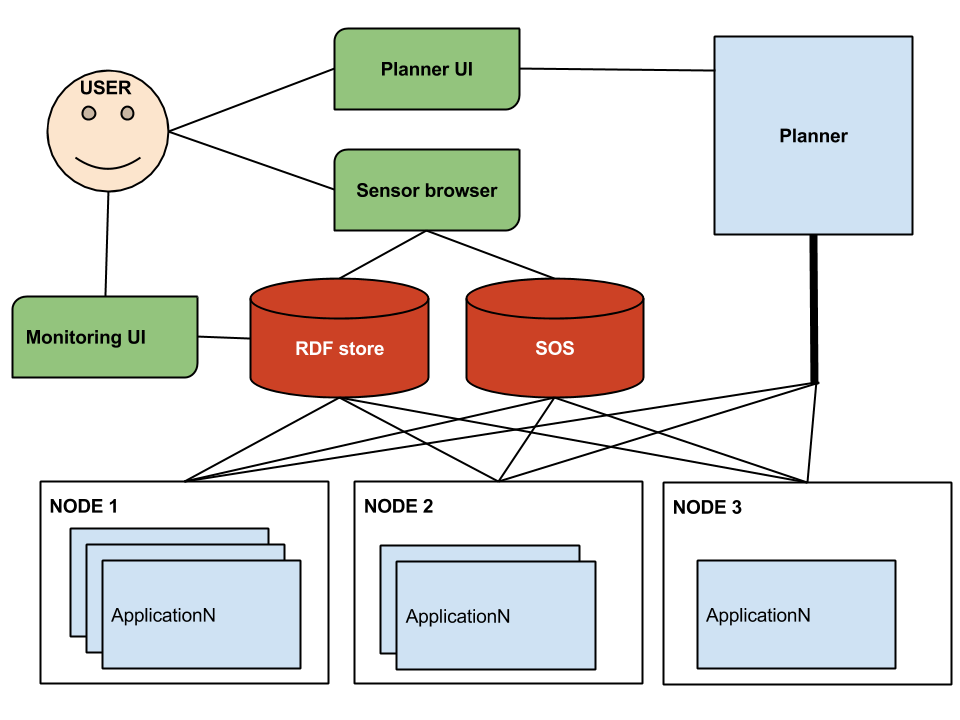
\includegraphics[width=0.6\textwidth]{figures/sysarch.png}
	\caption{System overview\label{fig:sysover}}
\end{figure}

\section{Sensors and resources}
The system is using different devices with different capabilities. There are simple microcontrollers and high performance mobile phones integrated in the system. 

The most simple solution is the Arduino Uno board with Ethernet controller. The card has an AVR based microcontroller working inside. It is good for simple measurement. It contains 14 general purpose inputs and outputs from which 6 can be PWM output. It's computing speed is 16Mhz.

The next in computational power is the Raspberry PI computer. This computer was designed to be cheap, reliable and compact, so poor people in developing countries can afford it. There are two models, both of them are fully working desktop computer with 700Mhz ARM cpu. It has:
\begin{itemize}
	\item 3 USB port
	\item 1 CSI port for raw camera input
	\item 1 Composite video output
	\item 1 HDMI output
	\item 1 SD/MMC/SDIO card reader
	\item 8 GPIO port (for UART, SPI, I2C, I2S audio)
\end{itemize} 
 It can run multiple operating systems, like Arch Linux, Raspbian OS, Debian, Slackware, etc. The more expensive model which costs around 35 dollars has a built in Ethernet port.  

The most expensive embedded computer is the BeagleBone in the project. This computer was developed by Texas instruments. It has a 600Mhz ARM Cortex 8 processor with 128 MB of RAM. It has built in features for sound and video processing. It costs around 150 USD. 

\section{The Sensor Observation Service}

The sensors communicate with the 52n SOS server using POX GET requests. To reach the service the sensors have to be in the same network or VPN to make the connection secure. The service has its own client installed next to it.

\section{RDF store}

The ontology is stored in an RDF database. It is based on the ontology introduced in the previous Chapter. The SSN Ontology has been extended for the custom use cases. The introduced ontology is called SISRO. It extends the original ontology in two ways:
\begin{itemize}
	\item It describes concepts and relations present in SensorML (and missing from SSN)
	\item It contains hardware details of the sensor devices
\end{itemize}


For easy communication with the sensors and the SOS server, the system can be reached using a custom service.
This Sensor Instance Semantic Registry Service contains the following interfaces:
\begin{itemize}
	\item Collection of Sensor Metadata. This interface contains the metadata for discovering sensors.
	\item System Discovery Interface. This interface is responsible for discovering sensors, searching in them using semantic connections.
	\item Sensor Status Interface. This interface manages the status information of the sensors. This interface makes it possible to search based on Status Information and change states.
	\item Sensor and hardware interconnection interface. Sensors does not have hardware description in SensorML. This interface supports application installation information and reconfiguration.
	\item SPARQL interface. This interface lets users to interact with the database on a low level.	  
\end{itemize}
The layer architecture can be seen on Figure \ref{fig:sisrserv}.	

\begin{figure}[h]
	\centering
	%custom
	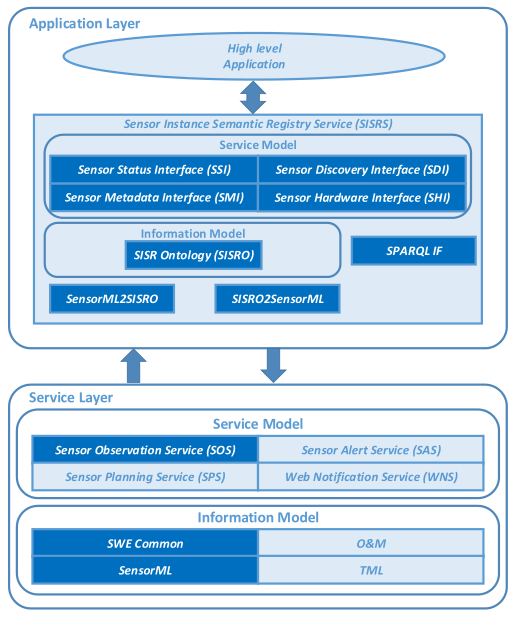
\includegraphics[width=0.6\textwidth]{figures/sisrserv.png}
	\caption{SISR service layers\label{fig:sisrserv}}
\end{figure}
The custom API has the following functions:
\begin{itemize}
\item GetCapabilities()
\end{itemize}
%----------------------------------------------------------------------------
\chapter{The monitoring system}
%----------------------------------------------------------------------------
\section{Goal of the implementation}

After introducing the data formats and the cyberphisical system implementation, in this part a sample application is shown that can handle connection to both data types.

The goal was to show how a connection can be created from third party applications. In further chapters the integration of the different types will be shown. The meaning of this phase is to seek for new ways to implement a web application using the connectors provided and measure the needs for such a web application. A whole test system was created to enable this.

\section{The test environment}

The system has been tested on multiple platforms. There was an Ubuntu Linux based virtual machine, which had a limited 512 MB of RAM, and a max. 10 GB storage. It's network card was hidden behind a NAT provided by the host computer. Java Runtime Environment was installed on the virtual machine for Stardog and SOS. For the web application NodeJS has been set up. 

The other platform was a Windows based computer. It had the same services (Stardog and SOS) running. The monitoring application requires NodeJs, which is a platform independent solution, so this did not mean any problem.

The chosen RDF database is Stardog Community edition. At first the software preallocates too much memory. It might be required for heavy weight applications but in our case it was not necessary.  The startup script had to be changed to make the software start. Changing this parameter does not decreases the performance significantly, compared to another computer with more memory. 

The chosen SOS server is 52north SOS 4.1 This is a recent release of the software. The used development version enables JSON communication. The server requires PostgreSQL database backend and Tomcat application server.

PostgreSQL 9.1.12 is used as the database backend for SOS. PostGIS environment had to be added. The database can be administrated using pgAdmin III from the host computer using port forward. For the Linux test environment no new users has been added, the SOS server uses the admin user to connect to the database. The database had to be created manually but tables and configuration is added during the installation automatically.

Tomcat 7 is installed to support SOS. To keep the system safe, on the Linux machine a new user is created to run the container and the application. The Stardog database is also running in a Tomcat like environment that is why it is started by the same user as the SOS server. 

\section{NodeJS: The backend of the monitoring application}

The connector application is written in JavaScript. This way the frontend and the backend application can be written using the same programming language. 
Since the V8 engine exists JavaScript can be compiled and run significantly faster\cite{v8} than before. 
The engine was introduced in 2008 and it caused a breakthrough in Javascript language. It has some new solutions that made V8 more effective, these are:
\begin{itemize}
\item \textbf{Hidden classes}: In V8 every object is a class. They are stored in a tree based structure and can be recalled faster.
\item \textbf{Dynamic Machine Code Generation}: V8 generates machine code from source without any intermediate bytecode language, like in Java.
\item \textbf{Inline cache}: It has a built in inline cache for resolving method names quicker.
\item \textbf{Efficient Garbage Collection}:Garbage collection freezes code execution and has a detailed map of the variable, however each garbage collection phase would only clear some part of the memory, it does not run full garbage collection every time.
\end{itemize}
NodeJS builds upon this V8 engine and lets JavaScript run on backend. Another advantage is that NodeJS has a single threaded, event driven core. This enables running applications faster, without worrying about thread safety. The architecture of the NodeJS environment can be seen on figure \ref{fig:node}. 
To keep the integrator separated a different user is added to run server side code on the Linux system. 
No web application container or web server is needed to run a NodeJS application. 
The software itself handles TCP connections and other modules help do it similar to Java Servlets. 
Because it has smaller overhead and dependencies, the created application should run faster than a rich Java Web application. 
NodeJS has an easy to use packaging system that makes dependency handling simple, like maven for Java. All necessary modules names are added to the related part of the package.json file and required packages are downloaded using the npm install command from a central repository. On the Windows machine a fork of NodeJS, the IOJS engine was tested. It is a community driven alternative that is fully compatible with NodeJS.
 
\begin{figure}[h]
\centering
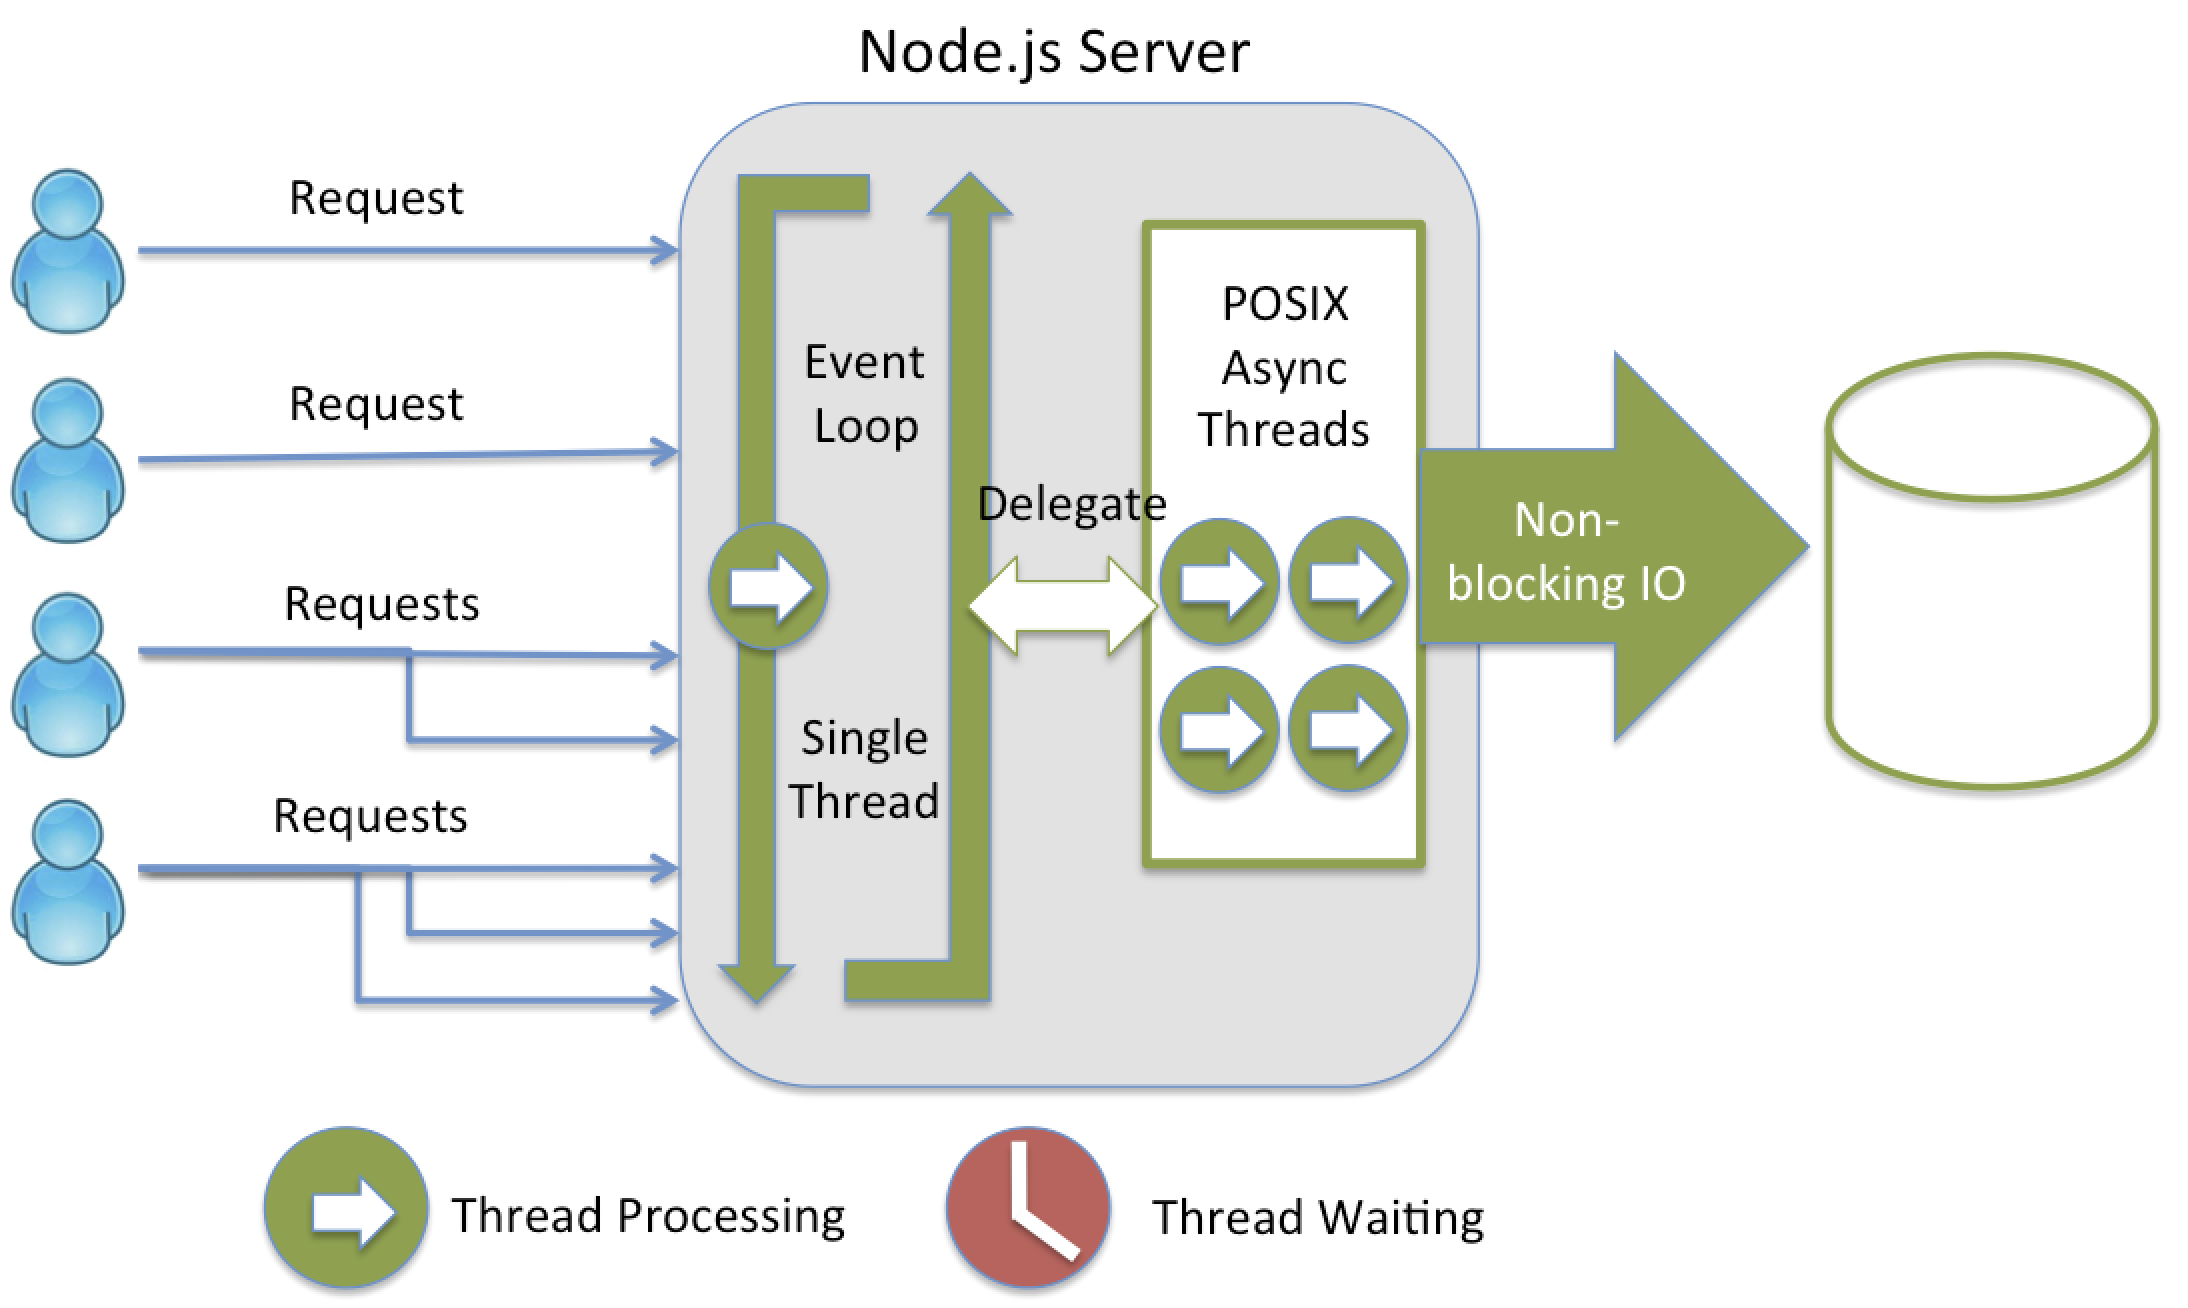
\includegraphics[width=0.6\textwidth]{figures/node.png}
\caption{NodeJS's event driven achitecture.\label{fig:node}}
\end{figure}

\section{Dependent modules}

Using the NPM (Node Package Manager) new dependent packages can be easily downloaded from a central  repository. NodeJS has a great coverage of packages, people can easily share their own modules. It contained 143 300 packages at the time of writing. In the implementation of the monitoring application there was a need for an interface for the database communication, interface for generating the web services and serving web pages. The most important packages were the following: 
\begin{itemize}

\item The ExpressJS module acts as the Servler engine for JavaScript. It handles incomming connections and parsed HTTP request are passed to a callback function which generates the responses. Different urls can have different callback functions to do routing. Express also supports many templating engines, like EJS or JADE.

\item Restler is an easy to use module that can asynchronously read a web page and parse it as JSON data and return it to the callback function. This can be used to communicate with the SOS server as it has an interface that is using JSON post requests to 
receive queries.

\item Stardog.JS is Stardog database servers own connector to get SPARQL queries. It is in early stages, however all the necessary functions are working. 

\item Nodemon, Forever or PM2 are utilities that run NodeJS codes automatically, restarts them on error or code changes. There is a support for development, that on any sourcecode change the changes are pushed to the browser without the need to refresh the browser. They can be configured to restart on error.
\end{itemize}

\section{AngularJS: the frontend of the monitoring application}

The ExpressJS module is serving the static files from the backend. The webpage itself is a single page web application which means that it consists of one html page and some partial pages that are loaded on the client side by a JavaScript framework. The framework that loads the different modules is called AngularJS. It was acquired by Google and now the project is maintained by them\cite{angular}. It's main advantage is that it implements a clear Model-View-Controller pattern. It dynamically changes the views, the HTML page based on the changes in the model, without additional coding.

For manipulating the user interface some external packages has been added to Angular. The most important of those are the following:
\begin{itemize}
\item \textbf{Chart.js}: This is a module that can be used to draw line charts or other kind of charts. This has an Angular integration and can be used to display the measured data in a time series plot. It can automatically smooth the curves. This is an open source project using HTML5.
\item \textbf{Angular Bootstrap DateTime picker}: This module has been chosen to select the time period to display. This is an open source project too.
\item \textbf{NG Tags Input}: This module can display tags in a search box and can handle autocomplete. 
\end{itemize}

For formatting the page the Bootstrap template is used. 
This library has some built in styles that are displayed the same in every browser. It has support for mobile devices.

\section{RDF representation of the SOS data}

\begin{figure}[h]
\centering
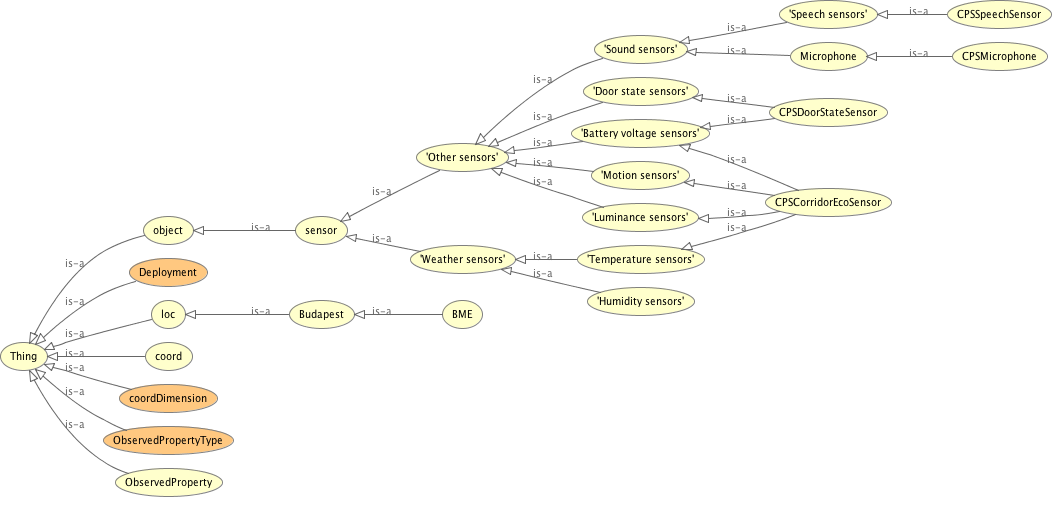
\includegraphics[width=0.6\textwidth]{figures/implrdf.png}
\caption{The Ontology used in the monitoring system.\label{fig:implrdf}}
\end{figure}

The general SISRO representation was missing some data of the example use case at the time of writing. To bridge this problem the monitoring application is using a different ontology that has been created to enable sensor browsing. This ontology contains only the necessary information to query sensor information. The elements can be seen on Figure \ref{fig:implrdf}. Some parts of the ontology hasn't been used in the monitoring system, the key components are:

\begin{itemize}
\item \textbf{Sensor}: This object is the ancestor of all sensor types. It has the Weather and Other sensors and their children. The instances of the child classes are the actual sensors. Figure \ref{fig:implrdf} shows that a final sensor can have multiple measurement, thus it can have multiple parents. Eco sensors are instances of the CPSCorridorEcoSensor and door state sensors are Instances of CPSDoorStateSensors. 
\item \textbf{loc}: This object stores location information, like URI of the feature of interest property in SOS and the name of the location. 
\item \textbf{ObservedProperty}: This is the observed feature of a sensor. There can be multiple observed properties for one sensor, like Battey voltage, Motion sensors, Speech text. The object instance contains the URI for the ObservedProperty in SOS and the type of the observed property.
\item \textbf{ObservedPopertyType}: This is the type of the observed property it has 3 instances in the example application: quantity, text, boolean.
\end{itemize}
 
The sensors of the use case are introduced in the end of the previous chapter, so those won't be covered here in details.
  
\section{Architecture of the monitoring system}

\begin{figure}[h]
\centering
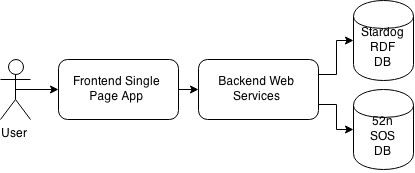
\includegraphics[width=0.6\textwidth]{figures/softwareArch.png}
\caption{Overall architecture of the monitoring system.\label{fig:overallarch}}
\end{figure}

The overall architecture can be seen on Figure \ref{fig:overallarch}. The user communicates through the single page web application. The web application dynamically loads the elements by sending requests to the backend service. The backend service connects to the two different databases and returns the data to the frontend. Initially the client side pages are also served by the backend service. 

\section{Architecture of the backend web service}

The backend services are called using HTTP POST and GET request. The POST body is always a JSON object. The detailed architecture of the backend services can be seen on Figure \ref{fig:backarch}.


\begin{figure}[h]
\centering
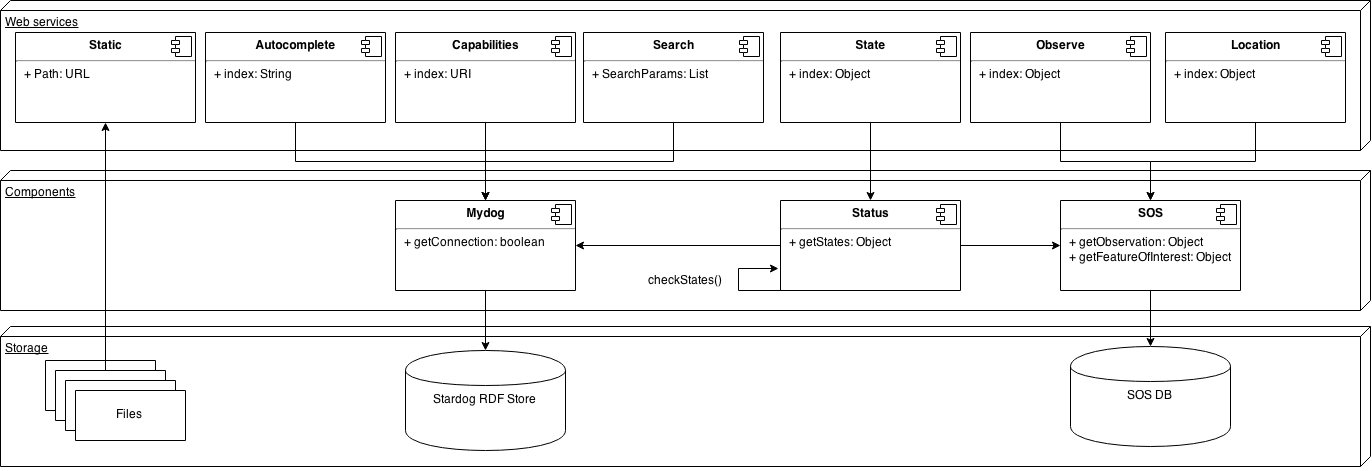
\includegraphics[width=0.6\textwidth]{figures/backendarch.png}
\caption{Detailed architecture of the backend services.\label{fig:backarch}}
\end{figure}

As the backend service is also providing the basic web server features, it has a built in static module, which in case there is no other web service by the provided location, it is serving a file from a given folder. If the file specified in the location does not exist the default index.html is returned. 
This ensures that Angular's custom routes are redirected to the same page. This feature is provided by ExpressJS.

In the sensor browser page, there is a search module where you can start typing in the name of the wanted category. After 3 letters a query is sent to the Autocomplete backend service which tries to find the matching categories and returns a list of the result. The Autocomplete module is using the Mydog module to get the data from Stardog. 
The query searches for every descendant of the sensor class and returns the result if found. The SPARQL query for that can be seen on Listing \ref{lst:autosparql}. 
\begin{lstlisting}[caption={SPARQL query for Autocomplete on the "wea" string\label{lst:autosparql}}]
SELECT ?name ?label {?name rdfs:subClassOf+ mit:sensor ; rdfs:label ?label. FILTER regex(?label, "wea","i")}';
\end{lstlisting}

The Capabilities module receives a procedure and returns all the information that describe the sensor in some way. This is similar to what SOS getCapabilities would return but with additional information. It is done using SPARQL in the RDF store. The result of this service call is used in other parts of the application. The SPARQL query for this can be seen on Listing \ref{lst:capsparql}. The result will be given as a JSON object. It will contain the sensor name, the procedure name, the offering of the procedure, the feature of interest of the procedure, the label of the feature of interest, the observed property URI, its name, and the name of the type of the observed property. 


\begin{lstlisting}[caption={SPARQL query for Capabilities\label{lst:capsparql}}]
SELECT ?label ?procedure ?offering ?foi ?flabel ?observable ?obs_name ?tlabel 
WHERE { <procedure/name> demo:procedure ?procedure ;
 rdfs:label ?label;
 demo:offering ?offering;
 demo:observedProperty ?obs ; 
 mit:hasLoc ?loc.
?loc demo:foi ?foi;
 rdfs:label ?flabel. 
?obs demo:observedPropertyURI ?observable ;
 rdfs:label ?obs_name ; mit:hasObservedPropertyType ?type .
?type rdfs:label ?tlabel}
\end{lstlisting}

The search module filters the sensor list. By default it will return the list of all sensors in the system. If there is an additional parameter list given in a given format the system will modify the query accordingly. This format is an array of  JSON objects which have three fields: 
\begin{itemize}
\item[text] The displayed name of the given parameter, it is not used.
\item[value] The class URI which identifies the class itself. This is added to the query.
\item[type] The type of the parameter. Yet it can have the value of "sensortype" only. 
\end{itemize}
The SPARQL query for retrieving the objects can be seen on Listing \ref{lst:searchsparql} The example SPARQL is using two categories for filtering. The result is always the union of the given categories. 

\begin{lstlisting}[caption={SPARQL query for Search\label{lst:searchsparql}}]
SELECT ?procedure ?name ?offering
    { ?class rdfs:subClassOf+ mit:sensor  .
     ?procedure rdf:type  ?class ; rdfs:label ?name ; demo:offering ?offering 
     { ?class rdfs:subClassOf* <category_one> } UNION { ?class rdfs:subClassOf* <category_two> }
    }
\end{lstlisting}

%TODO continue backend modules

%TODO describe frontend modules

%TODO write user manual
%----------------------------------------------------------------------------
\chapter*{Acknowledgement}\addcontentsline{toc}{chapter}{Acknowledgement}
%----------------------------------------------------------------------------

The author is thankful for Dr. Gy�rgy Strausz for managing the work and creating the necessary environment. The great help from Andr�s F�rh�cz about the semantic database and Csan�d Erd\H{o}s about the SOS database are also appreciated.

%\listoffigures\addcontentsline{toc}{chapter}{�br�k jegyz�ke}
%\listoftables\addcontentsline{toc}{chapter}{T�bl�zatok jegyz�ke}

\bibliography{mybib}
\addcontentsline{toc}{chapter}{Bibliography}
\bibliographystyle{plain}

%----------------------------------------------------------------------------
\appendix
%----------------------------------------------------------------------------
\chapter{Development and deployment}
\section*{Setting up the environment for development}
The project has been created in NodeJs and JavaScript. To compile or run it NodeJs or IOJS has to be installed on the system. The sources are sored in Github using git version control system. The backend development is using the Node's package manager, npm. The frontend is using bower package management. To build the whole system grunt-cli has to be installed. If both databases are installed the development steps for setting up the dev environment only are the following:
\begin{enumerate}
\item Install NodeJS or IOJS on the computer ( \url{https://nodejs.org/})
\item Install Git to be able to clone the project to the computer(\url{http://git-scm.com/})
\item Install Ruby for SASS ( \url{https://www.ruby-lang.org} )
\item Copy the project to your machine using git: \\
git clone https://github.com/djlancelot/dipterv-webapp.git
\item Install Node dependencies as administrator using command line: 
\begin{itemize}
\item \texttt{npm install -g grunt-cli}
\item \texttt{npm install -g bower}
\end{itemize}
\item Install SASS for compiling SCSS stylesheets using Rubies package manager \texttt{gem install sass}
\item Install local backend packages using \texttt{npm install} in the application folder
\item Install local frontend packages using \texttt{bower install}
\item Change the configuration in \texttt{server/config/environment} folder
\item Compile or run the code:
\begin{itemize}
\item Compile production version into dist folder using \texttt{grunt build --force} command
\item Run the application for testing as development version using \texttt{grunt serve} command
\end{itemize}
\end{enumerate}

The development environment will run on port 9000 and production version on port 8087 unless modified in server/config/environment directory.

If you need to add the RDF database dump to your Stardog instance you need to run \texttt{stardog data add --remove-all -v sont info/sensor-schema.rdf info/demo-sensors.rdf} inside the application folder. If the database is missing too it has to be created using \texttt{stardog-admin db create -n sont info/sensor-schema.rdf info/demo-sensors.rdf} command.

\section{Setting up the production version}

To run the application on a server you need to have Node or IOJS installed and a supervisor that can run the application. The application starts by running the \texttt{server/app.js} file. The environment has to be specified as an environment variable beforehand. The steps are he following:
\begin{enumerate}
\item Install NodeJS or IOJS
\item Copy the files from the dist folder (after compiling) to the destination computer to run production version. To run development version the contents of the original folder is needed, but production is preferred.
\item Install forever Node supervisor using npm install -g forever (on Windows you might also need npm insall -g forever-win)
\item Set Node environment variable to production (for production version only).
\begin{itemize}
\item On Windows you run \texttt{set NODE\_ENV=production}
\item On Linux simply add \texttt{NODE\_ENV=production} prefix before the forever start command
\end{itemize}
\item Start using forever with \texttt{forever start server/app.js}
\item Check if the application is running using \texttt{forever list} or the browser
\end{enumerate}
The production version will listen on port 8087.
\newpage
\section{Glossary}
\begin{description}
	\item[Audio stream] A series of network packets which transmit audio in a compressed format.
	
	\item[AVR microcontroller] A type of micro-controllers made by ATMEL Corporation. The microcontrollers are the main parts of an embeded system, they are one chip that has RAM, CPU, permanant store and input output peripherals embedded in one chip.
	
	\item[Backend] The server side, business logic based part of the application.
	
	\item[Cyberphisical system] a system that represents the physical world in the cyberspace. The measurements can be used to describe the world, run simulations and get predictions.
	
	\item[Frontend] The UI related part of an application.
	
	\item[GIT] Popular open source version control system. It is similar to SVN, except that all users have all the versions of the source code.
	
	\item[HTTP GET request] A basic HTTP request where the content of a specified URL is requested. Additional parameters may be appended to the URL.
	
	\item[HTTP POST request] This type of request is part of the HTTP standard. Using this kind of request the content is sent in the body of the request and not encoded in the URL of the request as in the GET requests.
	
	\item[JSON] JavaScript Object Notation is a format which describes JavaScript Object. Each object is given as a list of key value pair, where each value can be either a sub value or an array of values. Objects are written between curly brackets. Arrays are given in squared brackets, where values are divided by commas. The key and value is separated by a colon and those pairs are with a comma.
	
	\item[Maven] Dependency manager for JAVA packages. An XML descriptor provides information about dependencies which are automatically downloaded from a central repository. It can be used to customize the build process too.
	
	\item[NAT] Network address translation is a method to hide and transform queries from behind a router or gateway to the Internet.
	
	\item[PostgreSQL] Open source relational database system, It has many features compared to MySQL or other open source database systems.
	
	\item[PWM] Pulse-Wave-Modulation is a kind of signal processing when modulation is done by changing the duty cycle of a squared signal.

	\item[Tomcat]  Java Web application container. It runs Java WAR packages, provides dependency injection and some basic maintenance solutions. Can be easily expendable to support spring and databases.
\end{description}


\label{page:last}
\end{document}
